% =====================
% Chapter 4: Lists (Detailed)
% Audience: Architecture students new to coding
% =====================

\h{Lists}
A list in Python is a built-in, ordered, and mutable container that lets you keep many items in a single variable. For example, you could store every student’s age in one place like [18, 19, 20, …]. Lists play a role similar to dynamic arrays in other languages, but they can hold different data types in the same collection. You can add or remove items, change values, and access elements by their position; you can also take sublists to reorder or analyze parts of the data. Although a list can mix types, in practice you’ll usually keep items of the same kind for clarity. Because they’re flexible and efficient for everyday tasks, lists are one of the most important tools you’ll use as a Python developer.
\medskip
\begin{NoteBox}
\textbf{About this chapter.} Lists are Python's go-to ordered collection. You will use them to
hold spans per bay, room areas, wall layers, schedule rows, and more. This chapter explains how
to create, read, modify, sort, copy, and combine lists --- and how to avoid common pitfalls like
accidentally sharing the same list in many places.
\end{NoteBox}
\medskip

\begin{tcolorbox}[% passing options here
    title=Focus of this chapter:,
    colframe=orange,
    colback = white,
%    colback=orange!40!yellow!30, % think of mixing 2 colors with sliders
    arc=2mm % sharp corners
 ]
\begin{itemize}
    \item Creating lists and reading elements: Literals \c{[ ... ]}, heterogeneous items, indexing, negative indices, and slicing.
    \item Mutability and copying: In-place edits, shallow vs deep copies, and safe copy patterns (\c{list(a)}, \c{a[:]}, \c{a.copy()}, \c{copy.deepcopy}).
    \item Adding and removing items: \c{append}, \c{extend}, \c{insert}, \c{remove}, \c{pop}, \c{clear}; when each is appropriate.
    \item Searching and counting: \c{in}, \c{index}, \c{count}; handling \c{ValueError}.
    \item Sorting and reversing: In-place \c{.sort()} vs new list from \c{sorted()}, custom \c{key}, and \c{reverse=True}.
    \item Joining and splitting text: Using \c{",".join(...)} with \c{str} values and converting numbers via \c{map(str, ...)}.
    \item Iteration patterns: \c{for} loops, \c{enumerate}, \c{range}, list comprehensions (with conditions), and nested comprehensions.
    \item Unpacking and star expressions: \c{head, *body, tail} patterns; concatenation with \c{+} and repetition with \c{*}.
    \item Performance tips and pitfalls: Membership checks, list-of-lists replication trap, and method return values.
    \item Worked example and mini-lab: Realistic tasks on room schedules and spans.
\end{itemize}
\end{tcolorbox}

\hh{Why lists matter}
Why lists are the workhorse sequence: ordered, resizable, and mutable.


Lists are flexible: a single structure that can grow, shrink, and reorder items. In architectural
scripts you might keep a list of \emph{areas}, \emph{levels}, or \emph{materials}. Their mutability
lets you edit values in place as you refine a design.

\hh{Creating lists and indexing}
Literals \c{[...]} for creation, zero-based indexing, negative indices,
and slicing that returns new lists.


\code{c04_create}{python}{
    spans_m = [6.0, 7.2, 8.4]      # list of floats
    labels  = ["101", "102", "103"]# list of strings
    mixed   = ["A", 5, True]       # lists can hold mixed types (use sparingly)

    print(spans_m[0])              # first item -> 6.0
    print(spans_m[-1])             # last item  -> 8.4

    # slicing: [start:stop] (stop not included)
    first_two = spans_m[:2]        # [6.0, 7.2]
    tail      = spans_m[1:]        # [7.2, 8.4]
    every_other = spans_m[::2]     # [6.0, 8.4]
    print(first_two, tail, every_other)
}{Create lists, index, and slice.}

\begin{NoteBox}
\textbf{Tip.} Negative indices count from the end (\c{-1} last, \c{-2} second-to-last). Slices
return \emph{new} lists; indexing returns a single element.
\end{NoteBox}

\hh{List operations}
A list operation is any action performed on a Python list—creating, accessing, updating, removing items, searching, combining, or reordering. In short, these are the built-in tools Python provides to manage the items in a list. Figure \ref{fig:Listoperator} illustrates these operations; the next section explains each in detail.

\begin{figure}[htp!]
  \centering
  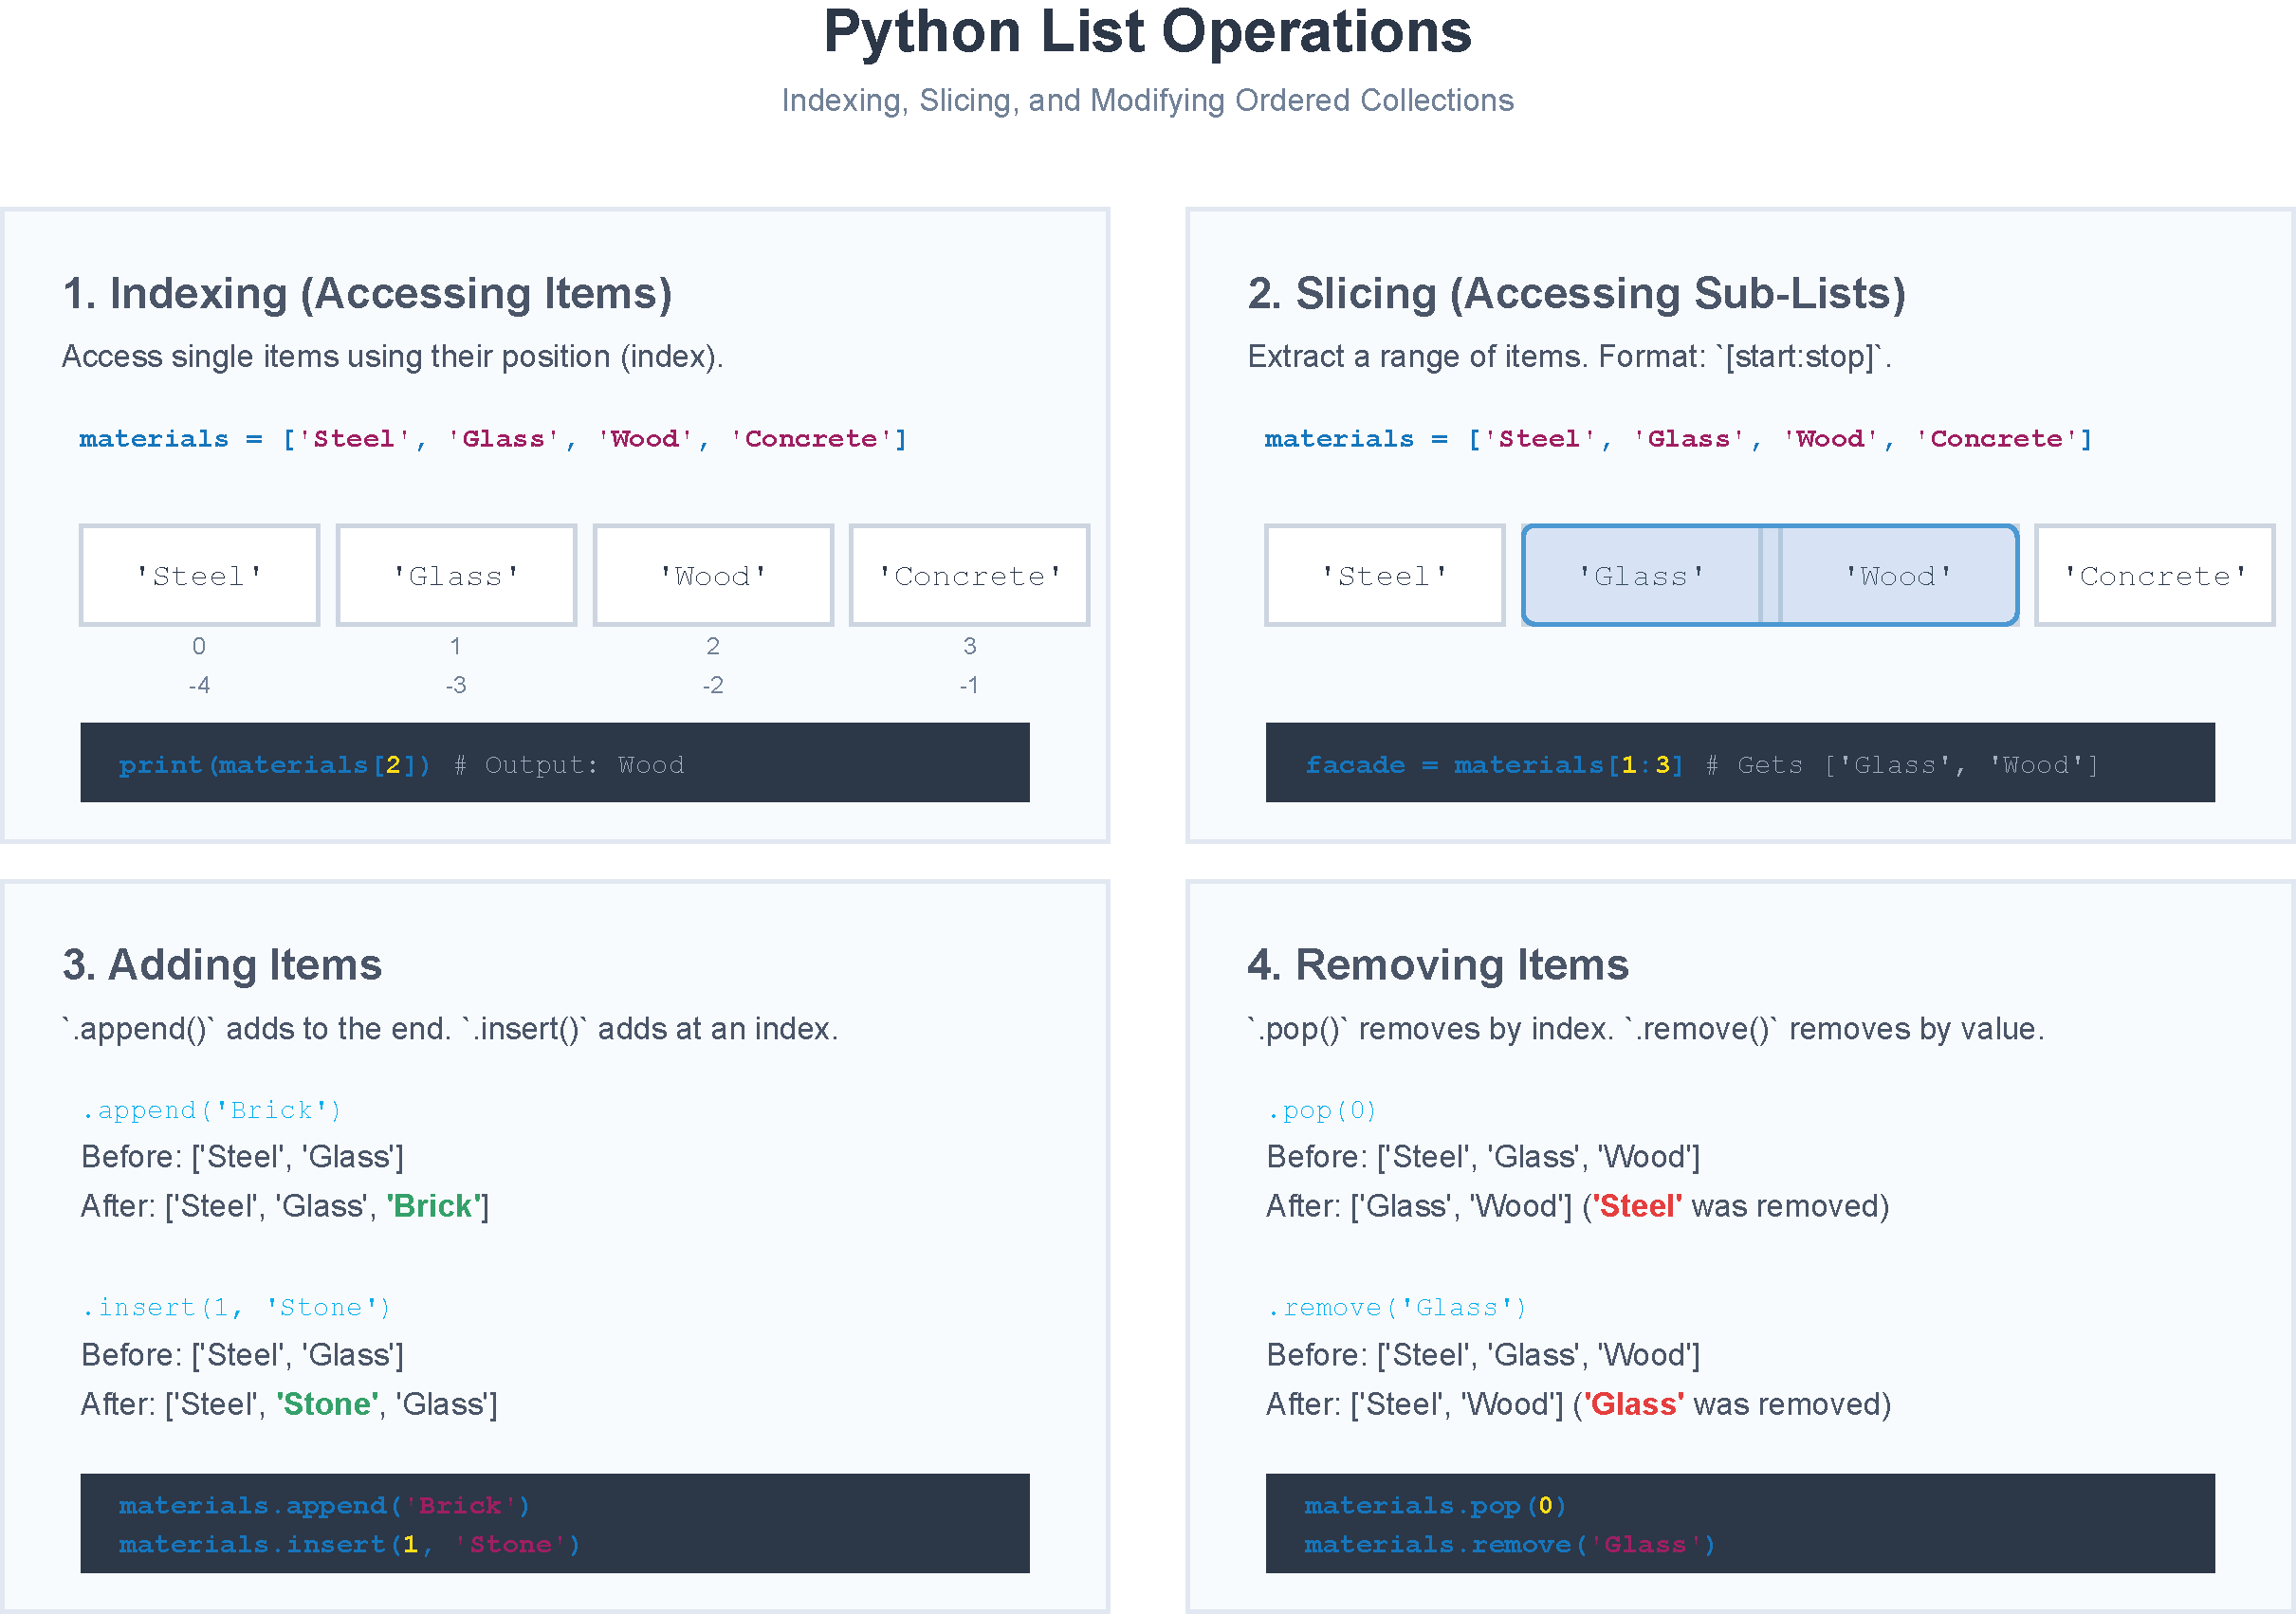
\includegraphics[width=\linewidth,keepaspectratio]{Figures/List/List_operator.pdf}
  \caption{Python list operations.}
  \label{fig:Listoperator}
\end{figure}

\hhh{Indexing (0-based) and Safe Access}

\begin{itemize}
\item Indexing uses \textbf{0-based} positions: first item is index \c{0}.
\item Negative indices count from the right: \c{-1} is the last item.
\item Accessing out of range raises \c{IndexError} — guard with \c{len()}.
\end{itemize}

\hhh{Slicing (start:stop:step) — Returns a {new} list}

\begin{itemize}
\item \c{start} inclusive, \c{stop} exclusive. Omitting means “from start” or “to end”.
\item Step lets you skip (\c{::2}) or reverse (\c{[::-1]}).
\item Slicing \emph{copies}; it does not change the original list.
\end{itemize}

\code{c04_index_slice}{python}{
    areas_m2 = [12.0, 9.5, 16.2, 10.0, 14.3]

    # Indexing
    print(areas_m2[0])    # 12.0 (first)
    print(areas_m2[-1])   # 14.3 (last)

    # Slicing (stop index is exclusive)
    print(areas_m2[:3])   # [12.0, 9.5, 16.2]  first three
    print(areas_m2[2:])   # [16.2, 10.0, 14.3] from index 2 to end
    print(areas_m2[1:4])  # [9.5, 16.2, 10.0]  middle slice
    print(areas_m2[::-1]) # reversed copy

    # Copying a whole list (shallow copy)
    copy1 = areas_m2[:]
    copy2 = list(areas_m2)
    copy3 = areas_m2.copy()
}{Index and slice patterns}

\hhh{Adding Items: {append}, {insert}, {extend}, {+}}

\begin{itemize}
\item \c{append(x)} adds one item at the end.
\item \c{insert(i, x)} adds at a position; shifts items right.
\item \c{extend(iterable)} or \c{+=} adds many items.
\item \c{+} creates a \emph{new} concatenated list.
\end{itemize}

\code{c04_add_remove}{python}{
    spans = [6.0, 7.2]

    spans.append(8.4)               # add one item at end
    spans.extend([7.2, 9.0])        # add many from another iterable
    spans.insert(1, 6.6)            # insert at position 1
    print(spans)                    # [6.0, 6.6, 7.2, 8.4, 7.2, 9.0]

    spans.remove(7.2)               # remove first matching value
    last = spans.pop()              # remove and return last item
    mid  = spans.pop(1)             # remove by index
    print(spans, last, mid)

    spans.clear()                   # remove all items
    print(spans)                    # []
}{Append, extend, insert, remove, pop, clear.}

\hhh{Removing Items: {pop}, {remove}, {del}, {clear}}

\begin{itemize}
\item \c{pop(i)} removes \emph{by index} and returns the item (defaults to last).
\item \c{remove(x)} removes the \emph{first matching value} (error if not found).
\item \c{del list[i]} deletes by index (no return); \c{del list[a:b]} deletes a slice.
\item \c{clear()} empties the list.
\end{itemize}

\code{c04_remove}{python}{
    rooms = ["R101", "R102", "R103", "R104", "R105"]

    last = rooms.pop()     # remove last; returns "R105"
    second = rooms.pop(1)  # remove by index; returns "R102"
    print(last, second, rooms)

    rooms.remove("R103")   # remove first matching value
    print(rooms)           # ["R101","R104"]

    dims = [3.2, 4.0, 2.8, 5.0, 2.4]
    del dims[0]            # delete first item
    del dims[1:3]          # delete a slice
    print(dims)

    dims.clear()           # empty the list
    print(dims)            # []
}{Remove by index, by value, by slice, or clear all}

\hh{Mutability and safe copies}
In-place edits vs copying. Use \c{a.copy()}, \c{a[:]}, or \c{list(a)} to avoid aliasing. Editing a list changes \emph{that} list. To avoid accidental sharing, make an explicit copy.

\code{c04_mutate_copy}{python}{
    bays = [6.0, 7.2, 8.4]
    bays[1] = 7.5                   # in-place edit
    print(bays)                     # [6.0, 7.5, 8.4]

    a = [1, 2, 3]
    b = a                           # reference copy: b points to the same list
    b.append(4)
    print(a)                        # [1, 2, 3, 4]  (a changed too)

    # safe (shallow) copies:
    c = list(a)
    d = a[:]                        # slice copy
    e = a.copy()                    # method copy
    d.append(5)
    print(a, d)                     # a unchanged, d has 5
}{In-place edits vs safe copying.}

\hhh{Shallow vs deep copies (nested lists)}
Shallow copies duplicate only the outer list; nested lists are \emph{shared}. Use \c{copy.deepcopy}
if you truly need independent nested structures.

\code{c04_deepcopy}{python}{
    import copy
    grid = [[1, 2], [3, 4]]
    shallow = grid[:]               # outer copied, inner lists shared
    deep    = copy.deepcopy(grid)   # fully independent

    grid[0][0] = 9
    print(shallow)                  # [[9, 2], [3, 4]]  changed
    print(deep)                     # [[1, 2], [3, 4]]  unchanged
}{Deep copy for nested lists.}

\begin{NoteBox}
\textbf{Errors to expect.} \c{remove(x)} raises \c{ValueError} if x is not present; \c{pop(i)} raises
\c{IndexError} if the index is out of range. Guard with \c{if x in lst} or check \c{len(lst)}.
\end{NoteBox}

\hh{Searching and counting}

Membership tests with \c{in}, finding positions with \c{index}, and tallying with \c{count}.


\code{c04_search}{python}{
    labels = ["101", "102", "101", "103"]
    print("102" in labels)          # membership -> True
    print(labels.count("101"))      # occurrences -> 2
    print(labels.index("103"))      # first index of value -> 3
}{Membership, count, and index.}

\hh{Sorting and reversing}
In-place \c{.sort()} vs \c{sorted()} new list, custom \c{key}, and \c{reverse=True}.
\begin{itemize}
  \item \texttt{list.sort()}: Think of this as an internal reorganization. This commands the list to sort itself. It \emph{mutates} the list in place and therefore returns \texttt{None}.
  \item  \texttt{sorted()}: Think of this as getting a sorted photocopy: you pass an iterable in, and you get a brand-new sorted list back. The original remains unchanged.
  \item \texttt{reverse=True} (descending order): By default, sorting happens in ascending order (smallest to largest). Set \texttt{reverse=True} to flip the final order (after applying \texttt{key}, if any). Works with both \texttt{list.sort()} and \texttt{sorted()}.
\end{itemize}
\code{c04_sort}{python}{
    areas = [18.5, 21.0, 17.2]
    areas.sort()                    # in-place sort (ascending)
    print(areas)                    # -> [17.2, 18.5, 21.0]

    areas.sort(reverse=True)        # in-place descending
    print(areas)                    # -> [21.0, 18.5, 17.2]

    # new sorted list (original unchanged)
    original = [('103', 18.5), ('101', 21.0), ('102', 17.2)]
    by_area = sorted(original, key=lambda r: r[1])
    print(original)                 # -> [('103', 18.5), ('101', 21.0), ('102', 17.2)]
    print(by_area)                  # -> [('102', 17.2), ('103', 18.5), ('101', 21.0)]

    by_room = sorted(original, key=lambda r: r[0])
    print(by_room)                  # -> [('101', 21.0), ('102', 17.2), ('103', 18.5)]
}{In-place sort vs sorted with key and reverse.}

\begin{NoteBox}
\textbf{Method returns.} \c{list.sort()} and \c{list.reverse()} return \c{None}. Use \c{sorted(lst)}
or \c{reversed(lst)} if you want a \emph{new} list instead of mutating the original.
\end{NoteBox}

\hh{Joining and splitting text}
The \texttt{.split()} method is a tool that belongs to strings. It breaks a single string into a list of smaller strings based on a specified “delimiter” or “separator.” Think of it like taking a sentence and breaking it into individual words. By default, if you don't specify a delimiter, \texttt{.split()} will use any whitespace (spaces, tabs, newlines) as the breaking point.

The \texttt{.join()} method does the exact opposite: it takes a list of strings and combines them into a single string, using a separator of your choice.
\begin{itemize}
  \item \textbf{\texttt{.split(sep=None)}}: Break a string into a \emph{list} of pieces.
    \begin{itemize}[label=\textcolor{blue}{--}, leftmargin=1.8em]
      \item Default \texttt{sep=None}: splits on any whitespace and collapses multiples.
      \item Give an explicit separator (e.g., \texttt{","}) to split on that character.
    \end{itemize}

  \item \textbf{\texttt{.join(iterable)}}: Join a list of \emph{strings} into one string, using \texttt{sep} in between.
    \begin{itemize}[label=\textcolor{blue}{--}, leftmargin=1.8em]
      \item The method is on the separator: \texttt{", ".join(parts)}.
      \item All items must be strings (convert numbers with \texttt{str()} or \texttt{map(str, ...)}).
    \end{itemize}
\end{itemize}

\code{c04_split_join_example}{python}{
    # A list of required materials
    materials_list = ["steel", "glass", "concrete"]

    # The string we want to use to join the items
    separator = ", "

    # Join the items in the list using the separator
    report_line = separator.join(materials_list)
    print(report_line)                  # -> 'steel, glass, concrete'

    # A string containing a list of project phases
    project_phases = "Schematic Design, Design Development, Construction Documents"

    # Split the string into a list using the comma and space as the delimiter
    phase_list = project_phases.split(", ")
    print(phase_list)                   # -> ['Schematic Design', 'Design Development', 'Construction Documents']
}{Join a list with \texttt{sep.join(...)} and split a string with \texttt{str.split(...)}.}


\hh{Iteration patterns}
Loops, \c{enumerate}, and comprehensions (with optional filters) for compact transformations.

\code{c04_iter}{python}{
    # A small dataset: bay spacings (meters)
    bays = [6.0, 7.2, 8.4]

    # 1) Plain iteration over the list.
    #    's' is the loop variable; it takes each value from 'bays' in order.
    for s in bays:
        print(s)
    # -> 6.0
    # -> 7.2
    # -> 8.4

    # 2) Index and value together with enumerate(...).
    #    enumerate(bays, start=1) yields (1, 6.0), (2, 7.2), (3, 8.4).
    #    Use start=1 for human-friendly numbering in printouts.
    for i, s in enumerate(bays, start=1):
        print("Bay", i, "=", s)
    # -> Bay 1 = 6.0
    # -> Bay 2 = 7.2
    # -> Bay 3 = 8.4

    # 3) List comprehension: transform each item.
    #    Read as: "for each s in bays, compute s*2, collect the results into a new list."
    doubled = [s * 2 for s in bays]
    print(doubled)                      # -> [12.0, 14.4, 16.8]

    # 4) List comprehension with a filter clause.
    #    Keep only values meeting the condition (s >= 7.0).
    long = [s for s in bays if s >= 7.0]
    print(long)                         # -> [7.2, 8.4]

    # 5) Nested comprehension (Cartesian product pattern).
    #    Evaluation order is left-to-right: for each w in widths, for each l in lengths.
    widths  = [3, 4]   # meters
    lengths = [5, 6]   # meters
    areas = [w * l for w in widths for l in lengths]
    print(areas)                        # -> [15, 18, 20, 24]
    #    Equivalent expanded form for clarity:
    # tmp = []
    # for w in widths:          # outer loop runs slower (w=3, then w=4)
    #     for l in lengths:     # inner loop runs faster (l=5, then l=6)
    #         tmp.append(w * l)
    # assert areas == tmp

    # Notes:
    # - List comprehensions create NEW lists without changing the originals.
    # - Prefer descriptive loop variable names in real code (e.g., spacing_m) for readability.
}{Looping with plain for, using enumerate, and building lists with comprehensions (transform, filter, nested).}


\hh{Unpacking and star expressions}
Split a list into head/body/tail; concatenate with \c{+} and repeat with \c{*}.

\code{c04_unpack_concat}{python}{
    # unpacking + concatenation/repetition (with outcomes)

    dims = [3, 4, 5, 6, 7, 8]

    # 1) Basic unpacking with a "rest" capture
    a, b, *rest = dims
    print(a, b, rest)              # -> 3 4 [5, 6, 7, 8]

    # 2) Everything except the last
    *first, last = dims
    print(first, last)             # -> [3, 4, 5, 6, 7] 8

    # 3) Head / body / tail
    *first, body, last = dims
    print(first, body, last)       # -> [3, 4, 5, 6] 7 8

    # 4) Exact-unpack all items (targets count must match)
    v, w, x, y, t, z = dims
    print(v, w, x, y, t, z)        # -> 3 4 5 6 7 8

    # 5) Head + middle + tail (capture the middle slice)
    head, *middle, tail = dims
    print(head, middle, tail)      # -> 3 [4, 5, 6, 7] 8

    # 6) Concatenation and repetition
    a = [1, 2] + [3, 4]
    b = [0] * 5
    print(a, b, rest, last)        # -> [1, 2, 3, 4] [0, 0, 0, 0, 0] [5, 6, 7, 8] 8

    # 7) Merge lists using * inside a literal
    left  = [10, 20]
    right = [30, 40]
    merged = [*left, *right]
    print(merged)                   # -> [10, 20, 30, 40]

    # 8) Star-unpack when calling functions (expands into positional args)
    print(*dims)                    # -> 3 4 5 6 7 8
}{Unpacking patterns, list concatenation/repetition, and related tips.}


\begin{NoteBox}
\textbf{Caution: list-of-lists replication.} \c{grid = [[0]*3]*3} creates \emph{three references}
to the \emph{same} inner list. Changing one row changes all rows. Prefer a comprehension:
\c{grid = [[0 for _ in range(3)] for _ in range(3)]}.
\end{NoteBox}

\hh{Performance tips}
Complexity basics: membership in lists vs sets, comprehensions vs append loops,
and avoiding front-insert patterns in tight loops.


\begin{itemize}
  \item Membership checks \c{x in big\_list} are O(n). If you only need membership, consider a \c{set}.
  \item Building a list with a comprehension is often clearer and at least as fast as appending in a loop.
  \item Avoid quadratic \c{list.insert(0, x)} in tight loops; appending at the end is O(1) amortized.
\end{itemize}

\hh{Worked example: sorting a room schedule}

\begin{NoteBox}
\textbf{What this section shows.} Extract fields with comprehensions and sort by one or more keys using \c{sorted(..., key=...)}.
\end{NoteBox}
\code{c04_worked}{python}{
    rooms = [
        {"room": "102", "area_m2": 21.0},
        {"room": "101", "area_m2": 18.5},
        {"room": "103", "area_m2": 17.2},
    ]

    # extract just the areas
    areas = [r["area_m2"] for r in rooms]            # [21.0, 18.5, 17.2]

    # sort rooms by area (descending), then by label
    rooms_sorted = sorted(rooms, key=lambda r: (-r["area_m2"], r["room"]))
    print(rooms_sorted)
}{Using list comprehension and sorted with key.}

\begin{minilab}
\textbf{Span cleanup and reporting (20 min)}\\
Given \c{spans = [6.0, 7.2, 7.2, 8.4, 6.0, 9.0]}, write code to:
\begin{itemize}
  \item Remove duplicates while preserving order.
  \item Report the count of each span (e.g., \c{6.0: 2, 7.2: 2, 8.4: 1, 9.0: 1}).
  \item Print a line like: \c{Spans (m): 6.0, 7.2, 8.4, 9.0}.
\end{itemize}
Hint: use a loop with a \c{seen} list (or a set for speed), plus \c{count()} for tallies.
\end{minilab}

\hh{Common pitfalls and how to avoid them}
Copying vs aliasing, \c{list.sort()} returning \c{None}, and the list-of-lists replication trap.

\begin{itemize}
  \item Assigning \c{b = a} does not copy the list; use \c{a.copy()} or \c{a[:]}.
  \item \c{list.sort()} returns \c{None}; do not write \c{new = a.sort()}. Use \c{sorted(a)}.
  \item \c{remove(x)} fails if \c{x} not in list; write \c{if x in a: a.remove(x)}.
  \item Replication with \c{*} duplicates references; use a comprehension for nested lists.
\end{itemize}

\hh{Self-check}
\begin{itemize}
  \item Show two ways to copy a list. Which one is shallow? When would you need \c{deepcopy}?
  \item Sort a list of dicts \c{[{"n": "A", "a": 12.0}, ...]} by \c{"a"} ascending, then by \c{"n"}.
  \item Turn \c{[6.0, 7.2, 8.4]} into the string \c{"6.0 | 7.2 | 8.4"}.
  \item Build a 3x3 zero grid correctly (no shared rows) in one line.
\end{itemize}

\hh{Quick reference: common list operations}

\begin{NoteBox}
\textbf{How to use this table.} Scan for the method/operator you need; prefer non-mutating forms when you must keep the original list.
\end{NoteBox}
\renewcommand{\arraystretch}{1.2}
\begin{table}[h]
\centering
\begin{tabularx}{\textwidth}{|l|X|X|}
\hline
\textbf{Operation} & \textbf{Example} & \textbf{Effect} \\ \hline
Create            & \texttt{a = [1,2,3]}                 & new list with three items \\ \hline
Index, slice      & \texttt{a[0]}, \texttt{a[-1]}, \texttt{a[1:]} & get element or sublist (new list) \\ \hline
Append, extend    & \texttt{a.append(4)}, \texttt{a.extend([5,6])} & add item(s) at end (in place) \\ \hline
Insert            & \texttt{a.insert(1, 99)}              & add at position 1 (in place) \\ \hline
Remove, pop       & \texttt{a.remove(2)}, \texttt{a.pop()}, \texttt{a.pop(0)} & delete by value / by index (returns item) \\ \hline
Count, index      & \texttt{a.count(2)}, \texttt{a.index(99)} & occurrences / first position \\ \hline
Sort, reverse     & \texttt{a.sort()}, \texttt{a.sort(reverse=True)} & order in place (returns \texttt{None}) \\ \hline
Sorted, reversed  & \texttt{b = sorted(a)}, \texttt{list(reversed(a))} & create new ordered list \\ \hline
Copy              & \texttt{a.copy()}, \texttt{a[:]}, \texttt{list(a)} & shallow copies \\ \hline
Join (strings)    & \texttt{' ,'.join(names)}             & build text from a list of strings \\ \hline
Comprehension     & \texttt{[f(x) for x in a if cond(x)]} & transform and/or filter into new list \\ \hline
\end{tabularx}
\caption{Common list operations at a glance.}
\end{table}
